\dictum[Thorin]{Is there no end to this accursed forest? Somebody must climb
a tree and have a look round. The only way is to choose the tallest
tree that overhangs the path.}

\begin{summary}
\item FluiDB expresses queries in relational algebra and defines
  reverse operations for most operations.
\item Query plan trees are accumulated in a bipartite DAG (QDAG) where
  the types of nodes are tables and bidirectional operations.
\item Queries are normalized to hashable objects (QNF) that abstract a
  wide range of rewrites. This allows efficient merging query plan
  trees into the QDAG.
\item Sub-graphs of the QDAG (clusters) represent higher level
  operations and are used as \emph{propagators} to infer information
  of the n-nodes like cardinality, column type, and uniqueness of
  subtuples.
\end{summary}

FluiDB is focused on query optimization and planning when the queries
in a workload being served can have common subqueries.  To exploit
these similarities between queries, FluiDB transforms them to
bipartite graphs of subqueries and bidirectional operators, which she
incrementally merges into a global query DAG and she uses to enumerate
the possible plans.  In this chapter, we will dive into how FluiDB
processes and merges these graphs. and into a detailed description of
the graphs themselves.

We will start by looking into what kinds of queries FluiDB can
understand and how she processes them. Then we will look at how she
relates the queries to each other to construct a tightly interrelated
story of the workflow by looking at the basic query graph, the heart
of FluiDB.

For manipulating a graph of queries, it is important that FluiDB can
distinguish between semantically different queries and and to be able
to tell when they are the equivalent.  We will look at how FluiDB
normalizes queries to efficiently determine this equivalence relation.

Then we will see how FluiDB organizes the nodes in the query graphs
into clusters representing single operations, how these clusters are
formed within the query graph, and how those are used to maintain
consistency among information about intermediate results.

Finally, we conclude by describing how the query processing
infrastructure interfaces with the rest of the components: the
planner, Antisthenis,and the code generator, described in later
chapters.

\section{Relational Algebra}
\label{sec:relational_algebra_semantics}

Much like most other RDBMSs, FluiDB deals with queries expressed in
terms of a \emph{relational algebra}.  Here we define the FluiDB
relational algebra semantics, that is, the traditional relational
algebra extended by unary operators for ordering \(s_e(X)\), limiting
\(l_i(X)\), anti-semijoin-ing \(\lnsemi\) and aggregating
\(\gamma_e(X)\), as listed in table \ref{tab:ra_sem}.

\begin{table}[H]
  \centering

  \begin{tabular}{lll}
    Description & RA & SQL\\
    \hline
    Aggregation & \(\gamma_e(X)\) & \sql{select * from X group by e}\\
    Ordering & \(s_e(X)\) & \sql{select * from X order by e}\\
    Limit & \(l_i(X)\) & \sql{select * from X limit i}\\
    Join & \(X \Join_p Y\) & \sql{select * from X, Y where p}\\
    Anti-semijoin & \(X \lnsemi_p Y\) & \\
    Union & \(X \cup Y\) & \\
    Selection & \(\sigma_p(X)\) & \sql{select * from X where p}\\
    Projection & \(\pi_r(X)\) & \sql{select r from X}\\
  \end{tabular}
  \caption{\label{tab:ra_sem}Correspondence between FluiDB's
    relational algebra expressions and SQL.}
\end{table}

Before going any further, it is important to clarify some assumptions
made to accommodate the design of FluiDB. Particularly that

\[\sigma_p A \cup \sigma_{\neg p} A \equiv A\]

This means that there no \sql{NULL} values are allowed since a
predicate over a \sql{NULL} value always evaluates to \hask{False},
breaking the double negation theorem. This allows the definition of a
bidirectional variant of the select (\(\sigma\)) operator.

Furthermore, we assume set semantics for all relations, meaning that a
valid relation needs to have at least one unique sub-tuple. The user
is not burdened with the responsibility of enforcing this, it is
rather enforced by a preprocessing stage on projections and
aggregations, exposing extra columns than the ones specified by the
user such that the resulting relation has at least one sub-tuple that
is unique for each row (see section \ref{sec:query_processing} on
query pre-processing).

The semantics of the sorting operation are preserved by making a small
concession to the set semantics: The \emph{only} time when records of
a relation are assumed by the planner to be ordered is for expressions
of the form \(s_e(X)\) and only for the duration between it running
and the next operation. In practice, this means that the FluiDB
planner generally treats \(s\) like an identity operation.

Besides these caveats, all operators known to FluiDB behave as expected.
The first of the extensions adopted is the antijoin operator
\(\lnsemi_p\) . It is equivalent to
\(A \lnsemi_p B \equiv A \backslash \pi_A(A \Join_p B)\) and it is
primarily useful for creating a bidirectional join by capturing the
rows left over from a join (see subsection \ref{sec:qdag} on the
QDAG). The important property we will be interested in is:

\[
  A \lnsemi_p B \cup \bar\pi_{cols(A)}(A \Join_p B) \equiv A
\]

\(\bar{\pi}_{cols(A)}\) meaning "group by the unique columns of \(A\)"
As syntactic sugar, we also define:

\[
  A \rnsemi_p B := A \lnsemi_{\neg p} B
\]

\subsection{Expressions}
\label{sec:expressions_predicates}

Relational algebra expressions contain expressions that operate at the
field level. These appear in projection column definitions, selection
predicates, aggregation column definitions, etc. These expressions are
organized in up to 4 nested layers based on the kinds of operators:

\begin{itemize}
\item The top layer is purely Boolean operations \hask{Prop} that
  can be rewritten in Cartesian normal form.
\item The intermediate layer \hask{Rel} describes relations between values
  (\(\equiv\), \sql{like}, \(<\), \(\le\), etc). This layer is not
  nested, i.e. we do not allow relations between relations.
\item The lowest layer \hask{Expr} is expressions of any kind that may
  return any value. The above layers can be expressed in terms of this
  layer to support the ternary operator \hask{if
    <expr> then <expr> else <expr>}.
\item The symbol layer describes the literal and symbolic atoms involved in the query.
  Its type is parametric in most parts of FluiDB to allow
  us to tag the symbols in the expression without breaking compatibility.
\end{itemize}

Predicates of selections and joins (joins are always \(\theta\) joins
at the type level) have type \hask{Prop (Rel (Expr e))} for some type
\hask{e} and projections have type \hask{QProj [(e,Expr e)]}. A
special layer is provided for aggregations \hask{Aggr} that makes it
possible to disallow nested aggregation functions at the type level
making the aggregation operator \hask{QGroup [(e,Expr (Aggr (Expr
  e)))] [Expr e]}, where the first argument of the constructor is the
aggregation functions and their names, and the sectond argument is the
expressions on which the grouping should happen.

The detailed definitions of the algebraic expressions are presented in
listing \ref{lst:expr_types}.

\begin{code}
  \begin{haskellcode}
    -- | Algebraic type of a proposition
    data Prop a = P2 BPOp (Prop a) (Prop a)
      | P1 UPOp (Prop a)
      | P0 a
    data UPOp = PNot
    data BPOp = PAnd | POr

    -- | Algebraic type of an expression
    data Expr s = E2 BEOp (Expr s) (Expr s)
      | E1 UEOp (Expr s)
      | E0 s
    data UEOp =
      EFun ElemFunction
      | ENot
      | EAbs
      | ESig
      | ENeg
    data ElemFunction
      = ExtractDay -- erased after parsing
      | ExtractMonth -- erased after parsing
      | ExtractYear -- erased after parsing
      | Prefix Int
      | Suffix Int
      | SubSeq Int Int
      | AssertLength Int
    data BEOp =
      -- Boolean (truthy)
      EEq | ELike | EAnd | EOr | ENEq
      -- Numeric
      | EAdd | ESub | EMul | EDiv

    -- | Algebraic type of a relation.
    data Rel a = R2 BROp a a
    data BROp
      = REq
      | RGt
      | RLt
      | RGe
      | RLe
      | RLike
      | RSubstring

    -- | Algebraic expression of an aggregation function
    data AggrFunction = AggrSum
      | AggrCount
      | AggrAvg
      | AggrMin
      | AggrMax
      | AggrFirst
  \end{haskellcode}
  \caption{\label{lst:expr_types} Types of algebraic expressions that compose the non-RA parts of the queries.}
\end{code}
%TODO: Definition of the query.
\section{QDAG: The unified query graph}
\label{sec:qdag}

The operation of FluiDB revolves around an AND-OR graph of relations
and algebraic operations, not unlike the ones commonly used in
multiquery optimization literature. This graph encodes all plans that
the query optimizer and planner will enumerate by means of
traversal. Said graph is a bipartite graph where \emph{t-nodes}
(similar to AND nodes in other literature) represent relational
operations and \emph{n-nodes} (similar to OR nodes elsewhere)
represent relations that will act as intermediate results.  A set of
extensions is introduced to the traditional AND-OR DAG to facilitate
the operation of FluiDB. In the interest of motivating those
extensions, we will take a very high level view of the operations on
the QDAG before describing them in detail.

There are multiple ways of composing relational operations to
materialize a certain relation. Each one is a relational algebraic
representation, we commonly refer to them as logical plans and they
are represented by trees similar to ASTs. These trees are made of two
kinds of nodes: operation nodes (t-nodes), and relation nodes
(n-nodes). For example, the query \(A \Join B \Join C\) may be
represented as \((A \Join B) \Join C\) or \(A \Join (B \Join C)\) due
to associativity of \(\Join\). Those two expressions represent two
tree forms where the join operators \(\Join\) are represented as
t-nodes and each of \(A\), \(B\), \(C\), \(A \Join B\), \(B \Join C\)
and \(A \Join B \Join C\) are represented as n-nodes.

While t-nodes can be triggered bidirectionally, they are not
symmetric: a subset of n-nodes are on the output side and another on
the input side. Each n-node can be materialized by \emph{triggering}
one of the input t-nodes, by running a connected operation to which
said n-node is on the output. It is clear then where the name OR-node
found in other literature originates: any of the input nodes may
participate to a plan involving the OR-node (n-node for
us). Conversely, each t-node can be triggered \(\iff\) all of it's
input n-nodes are materialized. Because \emph{all} input nodes must be
materialized, t-nodes are elsewhere referred to as AND-nodes. We
depart from the standard nomenclature to avoid confusion in the
presence of the extensions introduced by FluiDB. The planning of a
query amounts to searching for a sequence of t-nodes to be triggered
that would result in the corresponding node being materialized.

The QDAG of a query is created by unifying all logical plans that
would derive it by means of merging n-nodes that are equivalent. For
example the mentioned trees \((A \Join B) \Join C\) and \(A \Join (B
\Join C)\) shared the nodes \(A \Join B \Join C\), \(A\), \(B\) and
\(C\). A global QDAG is maintained by unifying the QDAG of each query
encountered into the global QDAG, again, by merging equivalent
n-nodes.

From a QDAG we can derive logical plans for queries. The planner
operates in terms of the global QDAG. It traverses the QDAG searching
for a plan (i.e., a sequence of t-node triggers) that will cheaply
materialize the requested node(s). This way, historical nodes can be
naturally considered. The problem of reusing materialized intermediate
results is thereby conceptualized as a graph traversal problem.

This technique is heavily inspired by multiquery optimization (MQO)
approaches like \cite{mistryMaterializedViewSelection2001} where they
use the AND-OR DAG to solve multiple queries simultaneously,
optimizing computation reuse.

QDAGs are different from AND-OR DAGs in a subtle but important way:
each t-node may have multiple outputs and can be partially
bidirectional. In other words, a t-node, as well as multiple inputs,
may have multiple outputs, any number of which may be materialized by
it being triggered. A \emph{reverse trigger} of said t-node would
materialize inputs provided that all outputs are materialized. Where
AND-nodes are similar to functions that when evaluated produce an
output given some input, t-nodes correspond to bidirectional relations
between sets of input and output relations.

% THIS IS THE IMPORTANT BIT!!! But it is buried in the text.
This not only creates opportunities in terms of what plans
are possible, but also opens the gate to a whole new regime for how
garbage collection is involved in the process of query planning. Any
n-node may potentially be garbage collected, even primary tables, as
long as the garbage collector can prove that it is reconstructable by
triggering or reverse triggering t-nodes. The storage budget is
thereby taken into account not only when selecting or rejecting
materialized views, but also while planning the query solution
itself.

To make this process clearer, as an example, consider a DAG that
contains just a selection in figure \ref{fig:just_a_selection} and a
more complete example of a QDAG involving multiple selection is
presented in figure \ref{fig:multiple_selections}

\begin{figure}[H]
  \begin{tikzdiagram}
    \tikzset{node distance=2cm}
    \tikzset{nnode/.style={ellipse,draw}}
    \tikzset{tnode/.style={rectangle,draw}}

    \node[tnode] (t) {\(\sigma_p\)};
    \node[nnode] (o2) [above left of=t] {\(\sigma_{\neg p}A\)};
    \node[nnode] (o1) [above right of=t] {\(\sigma_pA\)};
    \node[nnode] (i) [below of=t] {\(A\)};

    \path (t) edge (i);
    \path (t) edge (o1);
    \path (t) edge (o2);
  \end{tikzdiagram}

  \caption{\label{fig:just_a_selection}A selection t-node may generate
    both output nodes, \(\sigma_pA\) and \(\sigma_{\neg p}A\),
    rendering it a partition operation.}
\end{figure}

In the figures throughout this work we will denote n-nodes as circular
and t-nodes as squares or rectangles. When materializing
\(\sigma_p(A)\) the planner has the option of also materializing
\(\sigma_{\neg p}(A)\). If deemed beneficial \(A\) can be safely
deleted as the t-node can be reverse triggered to produce it. A
reverse trigger amounts to the union \(\sigma_{p}(A) \cup \sigma_{\neg
p}(A)\). It is generally assumed that any row not selected by \(p\) is
necessarily selected by \(\neg p\). To remind the reader of our RA
assumptions, this means that we do not support missing or \sql{NULL}
values as they break Boolean double negation. Furthermore, relations
are taken to be unordered sets of tuples.

\begin{figure}[H]
  \begin{tikzdiagram}
    \tikzset{node distance=2cm}
    \tikzset{nnode/.style={ellipse,draw}}
    \tikzset{tnode/.style={rectangle,draw}}

    \node[nnode] (i) {\(A\)};
    \node[tnode] (t_p) [above right=4cm of i] {\(\sigma_p\)};
    \node[tnode] (t_q) [above left=4cm of i] {\(\sigma_q\)};

    \node[nnode] (o2_p) [above left of=t_p] {\(\sigma_{\neg p}A\)};
    \node[nnode] (o1_p) [above right of=t_p] {\(\sigma_p A\)};
    \node[nnode] (o2_q) [above left of=t_q] {\(\sigma_{\neg q}A\)};
    \node[nnode] (o1_q) [above right of=t_q] {\(o_qA\)};

    \node[tnode] (t_pq) [above of=o1_p] {\(\sigma_{p \land q}\)};
    \node[nnode] (o2_pq) [above left of=t_pq] {\(\sigma_{p \land \neg p}A\)};
    \node[nnode] (o1_pq) [above right of=t_pq] {\(\sigma_{p \land q} A\)};

    \node[tnode] (t_qp) [above of=o1_q] {\(\sigma_{q \land p}\)};
    \node[nnode] (o2_qp) [above left of=t_qp] {\(\sigma_{p \land \neg q}A\)};


    \path (t_p) edge (i);
    \path (t_p) edge (o1_p);
    \path (t_p) edge (o2_p);
    \path (t_q) edge (i);
    \path (t_q) edge (o1_q);
    \path (t_q) edge (o2_q);
    \path (t_pq) edge (o1_p);
    \path (t_pq) edge (o1_pq);
    \path (t_pq) edge (o2_pq);
    \path (t_qp) edge (o1_q);
    \path (t_qp) edge (o2_qp);
    \path (t_qp) edge (o1_pq);
  \end{tikzdiagram}
  \caption{\label{fig:multiple_selections}Multiple selections can be
    composed to create larger networks.}
\end{figure}

In figure \ref{fig:multiple_selections} if \(sigma_{\neg p}A,\sigma_{q
\land p} A,\sigma_{p \land \neg q}A\) are all materialized, then \(A\)
is materializable as their union. This way \(\sigma_{p \land q} A\) is
readily available with no space overhead. Instead, the price paid is
that in the event that \(A\) is required, possibly in a different
context, constructing it requires the overhead of unioning all its
parts. Furthermore, there are two options for materializing \(\sigma_p
A\): either by selecting over \(A\), or via the union \(\sigma_{q
\land p}A \cup \sigma_{\neg q \land p}A\). Table
\ref{tab:reverse_corresp} demonstrates the correspondence between
relational algebra operators and the equivalence that enables their
reverse

\begin{table}[H]
  \centering
  \begin{tabular}{ll}
    Operator & Equivalence\\
    \hline
    Aggregation (\(\gamma_e(X)\)) & \(\bot\) \\
    Sorting \(s_e(X)\) & \(\bot\) \\
    Limit (\(l_i(X)\)) & \(l_i A \cup d_i A \equiv A\) \\
    Join (\(X \Join_p Y\)) / Anti-semijoin (\(X \lnsemi_p Y\)) & \( \bar{\pi}_{cols(A)}(A \Join B) \cup (A \rnsemi B) \equiv A\)  \\
    Selection (\(\sigma_p(X)\)) & \(\sigma_p A \cup \sigma_{\neg p} A \equiv A\) \\
    Projection (\(\pi_r(X)\)) & \(\pi_r A \Join \pi_{\bar{r}} A \equiv A\) \\
  \end{tabular}
  \caption{\label{tab:reverse_corresp}Each operation that may end up
    in the final result and the equivalence that ensures
    reversibility. \(\bot\) values indicate that the operator is not
    generally reversible.}

\end{table}

A concept closer to the functionality of t-nodes and n-nodes than AND
and OR nodes, and our very inspiration for this approach, is
\emph{propagators} \cite{radulPropagationNetworksFlexible2009a}. In
short, propagators are hyperedges in a hypergraph, the nodes of which
contain partial information about a value. Information about a value
can be accumulated from its neighbors. Each node can obtain at least
as much information about its value as the most precise neighbor. The
example provided in the paper is one of measuring the height of a
building by means of a barometer. One approach is timing the
barometer's free fall from the top of the building, another is by
measuring the length of the shadow of the barometer and comparing with
the length of the shadow of the building at the same time of day. One
may even use the barometer in its intended function and derive the
height of by comparing the difference in air pressure at the roof and
at the ground floor. Each of the mentioned methods will give very
noisy or partial information about the magnitude in question. In the
propagator paradigm, each of these measurements might be represented
as a node in a hyper-net. A propagator edge connecting these nodes
would combine information from all measurements and improve each of
the nodes' accuracy in their perception of the underlying value. A
t-node is similar to a propagator in that it does not have a strict
direction of information flow and can generate information on either
side given information on the other.

\subsection{Clusters and irreversible edges}

Generally, there is no one-to-one correspondence between
t-nodes and relational operators. Usually that is the case but
there is an exception: the join operator. As we made clear, a t-node
can generate any number of its inputs by reverse triggering it as
long as all of the outputs are materialized. Then one approach to
implementing a join operator might be:

\begin{figure}[H]
  \centering
  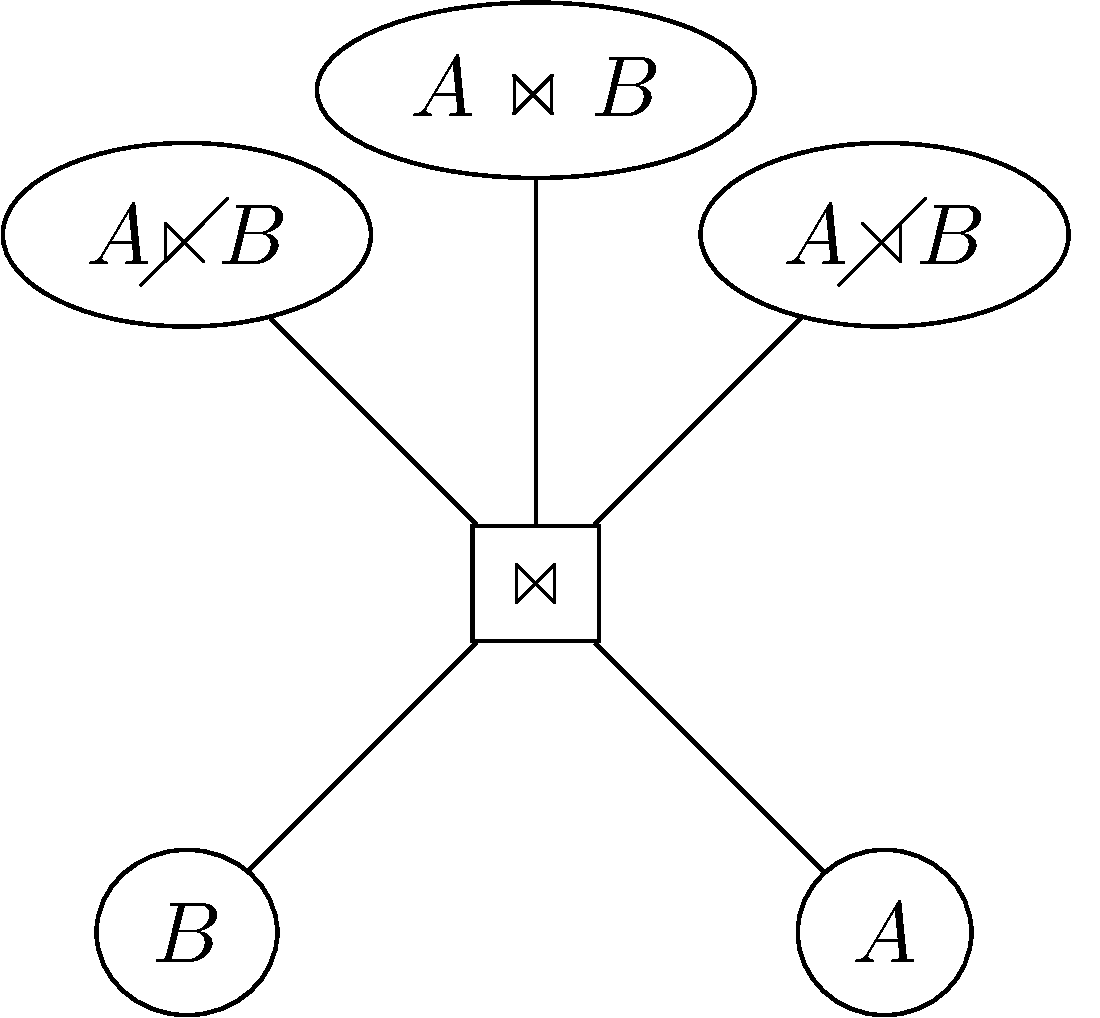
\includegraphics[width=0.5\textwidth]{./imgs/naivejoinnet.pdf}
  \caption{\label{fig:org78bb458}Representing a reversible join as a single t-node.}
\end{figure}

The \(\lnsemi\) operator is the antijoin operator, \(A \lnsemi B\)
includes the tuples in \(A\) that to not participate in \(A \Join B\). It
is the complement of the semijoin \(\lsemi\). Therefore

\[ \bar{\pi}_{cols(A)}(A \Join B) \cup (A \rnsemi B) \equiv A \]

\(\bar{\pi}_{cols(A)}\) means project on the columns of \(A\) group by
the unique columns of \(A\). Therefore, by having materialized \(\{A
\rnsemi B, A \Join B, A \lnsemi B\}\) we can create \({A,B}\) and vise
versa. We could, however be slightly more flexible than that, as we
might want to materialize \(A \rnsemi B\) but not \(A \lnsemi B\) to
the end of ensuring the materializability of only \(A\) and not
\(B\).

In this case neither the entire input nor the entire output are
materialized and yet all tables involved are materializable. To
overcome the limitation that this poses, we make the graph a bit more
complex and a bit more flexible by breaking the join into two stages
(see figure \ref{fig:joinnet}). First, we separate the join operands
(\(A\) and \(B\)) into the part that will be used in the join (\(A
\lsemi B\) and \(B \lsemi A\) respectively), and the part that will
not (\(A \rnsemi B\) and \(B \rnsemi A\) respectively) and then we
join only the useful parts \((A \lsemi B) \Join (B \lsemi A) \equiv A
\Join B\). Thus, we fundamentally break the 1-1 correspondence between
t-nodes and RA operators. Rather, operators correspond primarily to
\emph{clusters} of nodes. As we will see in detail in
\ref{fig:joinnet} the join cluster is the only multi-t-node cluster.

\begin{figure}[H]
  \centering 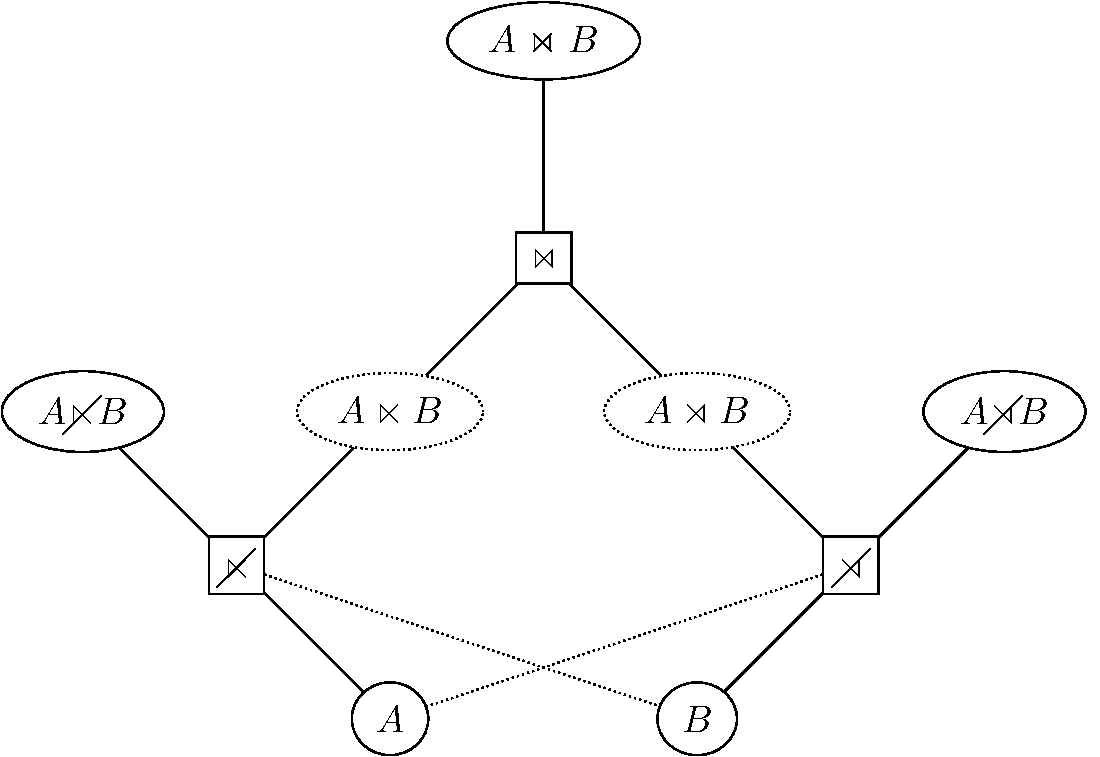
\includegraphics[width=.9\linewidth]{./imgs/joinnet.pdf}
  \caption{\label{fig:joinnet}The QDAG corresponding to a join is
    broken down in multiple t-nodes to facilitate greater
    flexibility.}
\end{figure}

The left antijoin node partitions \(A\) into \(A \lsemi B\) and
\(A \lnsemi B\), which is left semijoin in our null-less
context. Similarly for the right antijoin node which partitions \(B\)
to \(A \rsemi B\) and \(B \rnsemi A\). Joining the semijoin relations
\(A \lsemi B\) and \(B \lsemi A\) is equivalent to joining \(A\) and
\(B\).

In figure \ref{fig:joinnet} we used an antijoin t-node. From the
semantics of the antijoin \(A \lsemi B\) it is clear that no tuples
from \(B\) are included in either \(A \lnsemi B\) or \(A \rnsemi B\)
as \(B\) acts as a kind of predicate for selecting over \(A\). This
means that even though \(B\) is an input, there is no natural way of
creating \(B\) from the t-node's output. For these cases, we introduce
\emph{irreversible edges}. Remember that edges are always connections
between n-nodes and t-nodes. An irreversible input edge (a connection
from an n-node to a t-node) can only be used as an input to the t-node
and its n-node can \emph{not} be materialized by reverse triggering the
t-node.

Irreversible edges appear in the inputs of anti-join t-nodes but also
on the input of operations that cannot be information preserving,
notably aggregations. The output of an aggregation can not in general
be supplemented with extra information to reconstruct the input,
unless the entire input table is replicated. We therefore give up the
reversibility of such operations completely and mark the input edge as
irreversible. This is generally not a big problem as on the one hand
the results of aggregations tend to be small compared to the input
relations, and in the case of anti-join t-nodes, which are only found
in join clusters, for every anti-join node \(A \lnsemi B\) that is
unable to generate \(B\) by reverse triggering, there is a \(A \rnsemi
B\) that will happily generate \(B\) albeit refusing to generate
\(A\).

\begin{figure}[H]
  \centering
  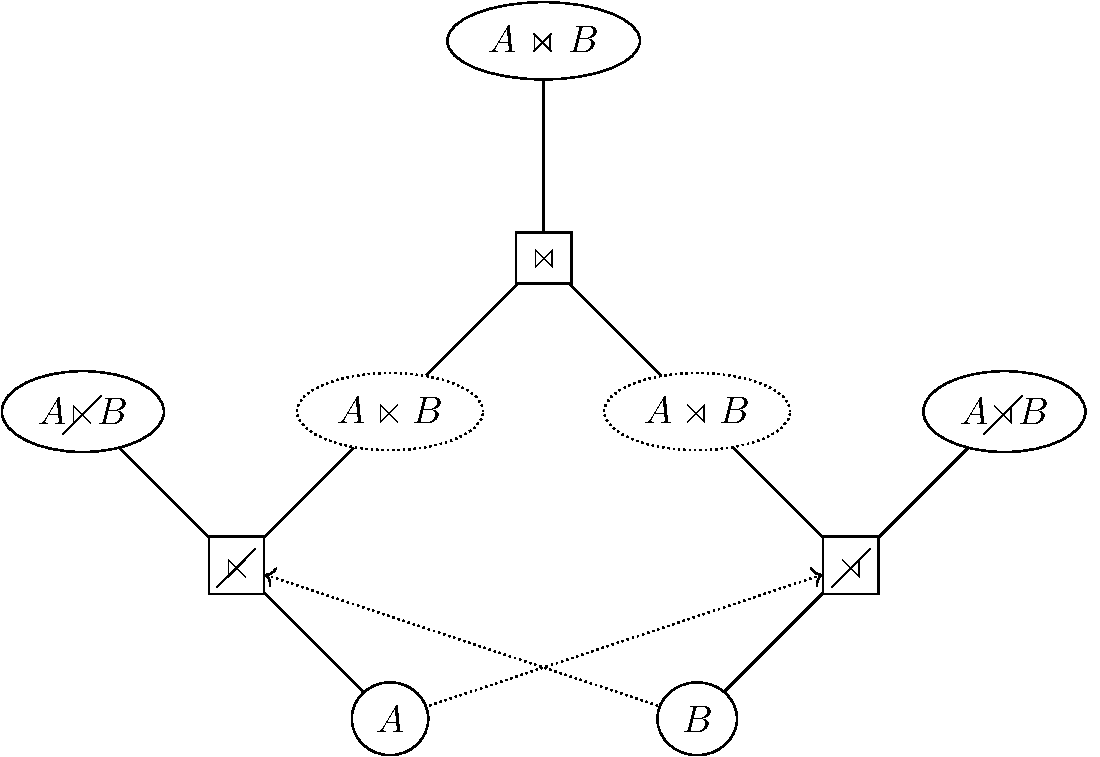
\includegraphics[width=.9\linewidth]{./imgs/joinnetdir.pdf}
  \caption{\label{fig:joinnetdir}The QDAG corresponding to a join is
    broken down in multiple t-nodes to facilitate greater
    flexibility.}
\end{figure}

\section{Deterministic query processing}
\label{sec:query_processing}

In this section, we will look at the initial steps of what happens
when FluiDB receives a query. Initially, the query is accepted in
textual form as SQL. Then it is sanitized to adhere to the properties
we defined for relational algebra and some trivial optimizations are
applied to remove artifacts of the parsing process. Finally, the query
is translated to a forest of possible join orderings. These are
rewrite-based optimizations that are deterministic and do not take
into account the rest of the workload.

\subsection{Query parsing}
\label{sec:query_parsing}

We use a custom library for parsing SQL queries into relational
algebra based on parser combinator monads
\cite{leijenParsecDirectStyle}. Our parser handles both the parsing
and decorrelation of the queries. In brief, parser combinators is a
functional interface to combining parsers to make larger, more complex parsers. A
parser \hask{p} has the form \hask{p a} which means that if the parser
is used to parse the matching text, it will return a result of type
\hask{a}. For this framework to work, two combinators are required:

\begin{itemize}
\item sequence (monadic bind) \hask{(>>=) : p a -> (a -> p b) -> p
    b} which sequentially tries two combinators and the latter one may
  use the result of the former.
\item the 'alternative' parser combinator \hask{<|> : p a -> p a -> p
    a} which tries one parser and if that fails tries another.
\item \hask{MonadGen e p} can generate a value of type \hask{p
    e}. Useful for creating names for unnamed expressions in
  projections, groups.
\end{itemize}

Simple parsers, like the \hask{parseInt} parser combinators, are then
combined to create more complex parsers (listing
\ref{lst:simple_parse}). This approach is fundamentally not dissimilar
to writing yacc files, but it is much more flexible as parser
combinators function as a domain-specific language that inherits all
the power of the host language, in our case Haskell.

\begin{code}
  \begin{haskellcode}
    parseInt :: MonadParse p => p Integer
    parseInt = do
      sign <- fmap (maybe 1 (const $ negate 1)) $ parseMaybe $ char '-'
      void $ parseMaybe $ char '-'
      (* sign) . read <$> readWhile isDigit

    parseSelectProj
      :: (MonadGen e p,MonadParse p)
      => p e -> p (Query e s -> Query e s)
    parseSelectProj eM = do
      word "select"
      fmap (Q1 . QProj) $ sep1 (word ",") $ do
      ex <- parseExpr (E0 <$> eM)
      parseMaybe (word "as" >> eM) >>= \case
        Just e -> return (e,ex)
        Nothing -> do
      e <- maybe pop (return . mkSymbol) $ asSymbol ex
      return (e,ex)
  \end{haskellcode}
  \caption{\label{lst:simple_parse}This parser returns a query
    modifier that is meant to be applied to a very simple product
    query generated by the \sql{from} clause. The actual selection
    parser is complex and handles many different cases, but it is
    built up from simple fundamental blocks.}
\end{code}

\subsection{Query prepossessing}

Immediately after parsing, the queries have several potential
inconsistencies with the notion of relational algebra that we
described in section \ref{sec:relational_algebra_semantics}.
For that reason, we implement an intermediate stage
where we rewrite the query to comply with various properties of the
RA, and which remove redundancies. In brief, those are the following:

\begin{itemize}
\item Projections and selections are squashed. For example
  \(\sigma_p\sigma_q\) becomes \(\sigma_{p \land q}\) and \(\pi_m
  \pi_{m'}\) becomes \(\pi_{m \circ m'}\).
\item Date intervals are translated to dates. This is because the
  physical planner does not handle dates specially so all dates and
  date intervals are converted to timestamps and second intervals. For
  example the expression \sql{date '2020-12-01' - interval '90' day} is
  immediately turned into \sql{date 2021-03-01}. Note that an
  expression like \sql{date '2020-12-01' + shipping_time} is not
  supported as it is not date arithmetic between literals.
\item Optimization of the \sql{like} operator: \sql{<VAR> like
    <STRING_LITERAL>} expressions where \sql{<STRING_LITERAL>} begins
  or ends with \texttt{\%} are turned into \hask{suffix_of} and
  \hask{prefix_of} expressions. For example, the expression \texttt{a
    like "\%.txt"} would be turned into \sql{".txt".suffix_of(a)}.
\item Substring expressions are turned into 0-indexed ones from
  1-indexed as is the case in SQL.
\item It is asserted that each intermediate relation has uniquely
  named columns. For example, there are necessarily name conflicts in
  \(A \Join A\).
\item It is asserted that sorting appears higher in the query AST than a
  selection, a join or an aggregation. All three of these operators
  affect the ordering of their inputs (see chapter 4 on code
  generation), and sort is the only operation that asserts tuple
  ordering on its output. Therefore \(s(A \Join B)\) is valid but
  \(s(A) \Join B\) is not.
\end{itemize}

Once the preliminary sanitization and simple optimization steps are
done we mark each instance of the primary table symbols with the
columns and their types. This is simply information derived by the
database schema. Then we do some processing and annotation on symbols
referring to symbols:

\begin{itemize}
\item First \emph{remap unique sub-tuples}. Each intermediate result,
  and each relation that we want to be able to reason about needs to
  have uniquely identifiable rows. For each relation in the QDAG we
  are keeping track of a set of columns, the unique sub-tuple, the
  combination of which is unique among each tuple of the same
  table. It is fairly straightforward to keep track of the unique
  subtuple for most operations, e.g., the unique sub-tuple of a
  Cartesian product or join is generally the concatenation of the
  unique sub-tuples of the input tables, the unique sub-tuple in the
  case a selection is the same as the unique sub-tuple of the input,
  in aggregations the unique sub-tuple is the same as the columns on
  which we aggregate, etc. The main challenge is projections and, in a
  similar manner aggregations, where it is possible that the operation
  does not project on the entire unique sub-tuple of the input. To
  mitigate this, we perform a pre-processing step to rewrite the
  projections to expose the entire unique sub-tuple. It is worth
  mentioning that there are cases where there are more than one
  combinations of fields that form a unique sub-tuple. We opt to keep
  track of all of them to have more flexibility in this
  pre-processing step: ideally we want to modify the projection as
  little as possible. In other words, we want to project as few extra
  columns as possible to keep the output table size as small as
  possible. As a simple example, the query
  \(\pi_{p\_color}\mathit{part}\) would become
  \(\pi_{p\_color,p\_partkey} \mathit{part}\).

\item Annotate each symbol referring to a column with the
corresponding primary table if there is one (named columns of
projections do not correspond to a primary table). This is useful both
in determining possible joins (as we will see in section
\ref{sec:possible_joins}) and in determining the types of
columns. This inference is sometimes trivial, for example, in the case
of references to columns of primary tables, or when annotating literal
values, but when references to columns of projections it is more
complex.  For example, in the query \(\sigma_{p(a)} \pi_{a \mapsto
f(X)}\), we need to infer the type of \(a\).  FluiDB will apply some
very simple heuristics to fake proper type inference. This is usually
enough to come up with accurate types as SQL's type system is basic.

\item Projection sharing is determined. As we will see in detail in
section \ref{sec:projection_algorithm} where we will be discussing the
implementation details of the projection algorithm and its reverse, it
is important that at least one unique tuple of a projection is shared
between a projection and its complement. At this stage, it is decided
which unique subtuple is to be shared and it is recorded in the RA
expression tree.
\end{itemize}

\subsection{Possible joins}
\label{sec:possible_joins}

Join ordering is one of the most detrimental optimizations of a query.
It is the selection of the associative order of joins.  The relation
\(A \Join B \Join C\) can be expressed as \((A \Join B) \Join C\) or as
\(A \Join (B \Join C)\).  Individual joins can have a wide range of
behaviors. From being similar to Cartesian products, being
prohibitively costly, and exploding the cardinality of the result; to
being similar to lookups, very cheap, and with a very small result.
Optimizers that process queries in isolation can aggressively push
down selections and prune the search space of join combinations when
they encounter expensive intermediate results.  FluiDB, however, needs
to keep track even of more expensive intermediate results as the high
cost may be amortized in the long run.

For this reason, at this stage we enumerate all possible join
permutations building a graph of all possible joins.

\begin{itemize}
\item All joins are turned into selection-products, so \(A \Join B\)
becomes \(\sigma(A \times B)\)
\item selections are pulled up and merged, (\(\sigma_p \sigma_q A\)
becomes \(\sigma_{p \land q}\))
\item products are represented as sets of relational algebraic
expressions.
\end{itemize}

Then all possible permutations of joins are created. For example
\(\sigma_{a=b \land b=c}(A \times B \times C)\) becomes \(\{(A
\Join_{a=b} B) \Join_{b=c} C, A \Join_{a=b} (B \Join_{b=c} C)\}\).

Note that we do not include queries that are only different
w.r.t. commutativity, i.e., we don't include both \(A \Join B\) and
\(B \Join A\). This part of FluiDB depends on the consumer of the data
structure to disambiguate between them. Another caveat is that since
Cartesian products are very large and are almost never used in the
actual plans, an option that disallows product intermediate results is
enabled by default. Therefore, in our example we prune relations like
\(\sigma_{a=b}((A \times C) \Join_{b=c}B)\). Furthermore, allowing
Cartesian products exponentially explodes the space of possible plans
to a degree that makes the resulting data structure virtually
unusable.

Once selections are merged, we find product trees, i.e., contiguous
parts of the tree that only contain Cartesian products, and combine them
into multi-sets of subtrees such that \(\sigma(C \times (A \times B)
\times D)\) becomes \(\sigma(\{A,B,C,D\})\).

Then selection propositions are normalized to conjunctive normal form
and into sets. For example \(\sigma_{p_1 \lor (p_2 \land p_3)}A\)
becomes \(\sigma_{(p_1 \lor p_2) \land (p_1 \lor p_3)}A\), and in fact
the conjunctive terms are also represented as sets of subterms, so the
final form would be better expressed as \(\sigma_{\{p_1 \lor p_2,p_1
\lor p_3\}}A\). This leaves us with a tree of terms of the form
\(Q[\sigma_{\{p_0,p_1,...,p_l\}}\{Q_0,Q_1,...,Q_k\}]\) where each term
\(p_i\) refers to columns in one or more \(Q_j\) relations and
\(Q[\cdot]\) is a query tree with \(\cdot\) as a subtree. We will
refer to such a selection-product pair as an SP-term.

To turn this representation into a forest, we will turn each SP-term
into a set of regular join trees, the Cartesian product of which will
yield the possible joins. We summarize the process as follows:

\begin{itemize}
\item We iterate over all pairs of sub-multisets into which the
  multiset \(\{Q_0,Q_1,...,Q_k\}\) can be split. We follow each of the
  following steps for each of the resulting sub-multisets.
\item We split the \(p\) terms in three parts depending on which
  sub-multiset of relations their symbols refer to. One set are terms
  where the columns mentioned refer \emph{only} to the left
  sub-multiset (left \(p\)-terms), another set are terms where columns
  mentioned refer \emph{only} to the right sub-multiset, and the rest
  (right \(p\)-terms) must necessarily have references to columns of
  \emph{both} sub-multisets. We call the latter category
  \emph{connector \(p\)-terms}.
\item We turn each side of the split into an SP-term by associating it
  with the left and right \(p\)-term set. We repeat the process of
  generating join trees out of each SP-term created and connect them
  in an all-to-all fashion by creating theta joins using the
  conjunction of the connector \(p\)-terms. In case the the set of
  connector \(p\)-terms is empty, that would mean that the connection
  of the join trees must be done with a Cartesian product. As
  mentioned above, we want to avoid inserting Cartesian products in
  our graph so we reject those cases outright. Optionally, we may even
  want to reject all non-natural joins altogether, unless that would
  mean eliminating all possible plans.
\end{itemize}

The fundamental forest structure of literally collecting each logical
plan individually is highly redundant. Therefore, we abstract away the
redundancy by representing the forest as a \emph{bipartite tree}.

\begin{itemize}
\item One kind of node represents a plan fragment, or a \emph{sub-tree}
\item The other kind represents a forest of semantically equivalent
  subtrees earmarked with a unique hash for them. The fact that the
  subtrees are semantically equivalent means that they
  evaluate to the same data. They therefore have the same normal form
  as discussed in section \ref{sec:qnf} on  Query Normal Form (QNF). Finding the normal form
  hash of one would mean the normal form hash of the rest. This will
  prove useful when inserting this structure in the graph. We refer to
  these as \emph{sub-forests}.
\end{itemize}

In other words, the relational algebra tree is interleaved with
OR-nodes of different representations of the subquery. For example
\(\gamma(\sigma_{a=b \land b=c}(A \times B \times C))\) becomes
\(\gamma\{A \Join_{a=b} B) \Join_{b=c} C, A \Join_{a=b} (B \Join_{b=c}
C)\}\). This way we mitigate the combinatorial explosion of interleaved
nesting joins with other operations.

The algorithm for building the forest out of the pre-processed query
is described in listing \ref{lst:possible_joins}.

\begin{code}
  \begin{pycode}
    def possible_joins(q):
        # Split a query that is equvalent to
        # sel(p1 and p2 and p3 and ..., prod(q1, q2, q3,...))
        # into
        # [p1,p2,p3,..], [q1,q2,q3,...]
        and_props,subqueries =  as_prod(q)
        
        # If the query is product just reject it.
        if len(and_props) == 0 and len(subqueries) > 1:
            return
            
        # if the query is not a join get the possible joins of the subqueries.
        if len(and_props) == 0 and len(subqueries) == 1:
            yield q.map_children(possible_joins)
            return 
              
        # All possible partitions where the partitions are non-empty
        for lqs,rqs in possible_partitions(subqueries):
            # has_free_vars(p,[q1,q2,q3...]) checks if all the atoms in p
            # are either literals or columns in one of the q1,q2,...
            
            # The props that can be pushed in the left partition
            lps = filter(lambda p: not has_free_vars(p,lqs), and_props)
            # The props that can be pished in the right partition
            rps = filter(lambda p: not has_free_vars(p,rqs), and_props)
            # The props that connect the partitions into a join.
            jps = filter(lambda p: has_free_vars(p,lqs)
                         and has_free_vars(p,rqs),
                         and_props)

            # If there are no predicates connecting it is product. We
            # disallow products.
            if len(jps) == 0: continue

            # A valid join to be considered while planning!
            lq = sel(lps,prod(rqs))
            rq = sel(rps,prod(rqs))
            yield join(jps,possible_joins(lq), possible_joins(rq))
  \end{pycode}
  \caption{\label{lst:possible_joins} Pseudo-python description of
    finding all possible joins. For clarity, it is abbreviated to omit sanity
    checking, memoization, some type conversions, etc.}
\end{code}

It is worth stressing that many of the subtrees generated this way
will be equivalent. As analyzed in \cite{bibtexa} and discussed in
section \ref{sec:qnf}, in pure functional settings like our, DAGs can
have explosive complexity during traversal. Even worse in this case
even the space complexity can indeed be needlessly exponential. For
that reason we maintain a hash map matching hashes with the
corresponding matching subtrees. Before inserting a newly created
forest into our structure, we perform a lookup in the hash map. If we
find something we throw away the newly created forest for the
optimizer runtime's garbage collector to recycle, and we use the one
in the hash map instead. Otherwise, we insert our forest both in the
hashmap and in the tree. This way we deduplicate our data structure to
some degree. Furthermore, in the same vain as \cite{bibtexa} we
earmark all our forests with their hash so we do not have to traverse
them again to compute it. The result of this is that in total we
completely traverse the forest once, in order to compute the hashes of
each sub-forest and then we use those hashes to test sub-forests for
equality.

\section{Query Normal Form (QNF)}
\label{sec:qnf}

It is imperative that the QDAG has as little redundancy as possible,
two subqueries that describe the the same relation should be
represented as the same node. Equivalence of RA expressions is
infamously NP-complete
\cite{sagivEquivalencesRelationalExpressions1980} but we make a best
effort to normalize queries such that they are hashable and comparable
via simple structural equality. The core of normalization is
transforming the queries to Cartesian normal form

\[
  \zeta_{x_1}(A) \Join_{p_1} \zeta_{x_2}(B) \Join_{p_2} \zeta_{x_3} (\sigma_{p_3}(C)) \to \zeta_{x_1;x_2;x_3}(\sigma_{p_1 \land p_2 \land p3}(A \times B \times C))
\]

where \(\zeta \in \{\pi,\gamma\}\).

\subsection{QNF Structure}

FluiDB's Query Normal Forms are highly polymorphic data structures
separate from RA data structures. The general QNF form can encapsulate
one of several special forms, all of which strive to abstract away as
many valid RA rewrites as possible, and ideally achieve a one-to-one
correspondence between a QNF and a table. While the QNF in its general
form (listing \ref{lst:qnf_struct}) is specialized to represent
several different forms internally to the QNF subsystem, outside of it
there are two main objects:

\begin{itemize}
\item The normal form of a relational algebra query
\item A column of a normal-form query.
\end{itemize}

\begin{code}
  \begin{haskellcode}
    data QNFQuerySPDCF sel_f prod_f dbg_f col_f f e s =
      QNFQuery
      { qnfColumns :: col_f (QNFProj f e s) (QNFAggr f e s)
        -- ^ What columns kept. Each of these is a column of
        -- QNFProd.
        ,qnfSel :: sel_f (QNFSel e s)
        -- ^ And conjuction of selection.
        ,qnfProd :: prod_f (QNFProd e s)
        -- ^ `QNFProd e s` is a set of multiple rewrites of a single
        -- relation. Essentially {Query (..) (QNFQuery e s)}. Each element
        -- of this set needs to have the same set of QNFQuery's. The binary
        -- operators allowed here MUST expose plans from ONE side. Otherwise
        -- the qnfColumns will be ambiguous. In practice only Product/Join
        -- expose both sides but if there are more in the future know that
        -- qnf machinery will break.
        ,qnfOrigDEBUG' :: dbg_f (Query e s)
        -- ^ The original query expression for debugging purposes.
        ,qnfHash :: QNFKey e s
        -- ^ Cache the hash. Hashing is done separately for each field so we
        -- don't recompute hashes of unchanged fields after each operation.
      }
  \end{haskellcode}
  \caption{\label{lst:qnf_struct}The QNF datastructure.}
\end{code}

In section \ref{sec:building_qnfs} on building QNFs,
we will look at several specializations that are useful as intermediate. In this
section we will focus on each of the fields of the \hask{QNFQuery}
constructor.

\subsubsection{QNF Product collection}

The \hask{qnfProd :: prod_f (QNFProd e s)} field contains the
unordered collection of subqueries \(\{A_1,... , A_n\}\) in the
equivalent \(\pi \sigma (A_1 \times ... \times A_n)\), typically as a
hash-set (via the instantiation of \hask{prod\_f} as
\hask{HashSet}). Each of the \(A_i\) terms may be one of the following:

\begin{itemize}
\item A primary table
\item A QNF with an opposite kind \hask{qnfCol} (if \(Q\) is a
  projection an \(A_i\) may be an aggregation)
\item A set of equivalent RA expressions that are not reducible to the
  \(\pi \sigma(A_1 \times ... \times A_n\), for example \(\{A \lnsemi
  B,B \rnsemi A\}\) or \(\{l_N(A)\}\)
\end{itemize}

Focusing on the latter case, there are certain equivalent rewrites
that are not easily expressible in the QNF. For that reason instead of
perpetually extending the QNF system we provide this expensive method
of simply enumerating equivalent queries in RA form. These RA queries
have at the leaves of the expressions either QNFs or primary
tables. The only restriction that we place on these queries is that
the schema of the inputs is simply forwarded to the output without
modification of the individual fields so that the \hask{cnfCol} vector can
refer directly to them.

\subsubsection{QNF Columns, projections and aggregations}
\label{sec:qnf_proj_aggr}

The \hask{qnfColumns :: col_f (QNFProj f e s) (QNFAggr f e s)} field
indicates which columns are exposed by the query. There are two kinds
of column sets: aggregated columns and projected columns. Depending on
the context \hask{col_f} is instatiated to a type that allows the
column to be \emph{always} aggregation, \emph{always} projection, or
either of the two.

Whenever a \hask{QNFQuery} is found outside of the QNF sub-module
\hask{col_f} will be instantiated as \hask{Either}, which is to say
that a query may be an aggregation (\hask{Right}) or a projection
(\hask{Left}). A query with no explicit projection operand at its root is
translated to QNF by enumerating the columns into this field. In all of
these storing them in a container of parametric type \hask{f}, which is
the main distinguishing factor between QNF columns and QNF queries: a query
projection exposes an unordered bag of columns through the projection/aggregation
field (\hask{f} is instantiated to \hask{HashBag}) while a QNF column exposes
\emph{exactly one} column (\hask{f} is instantiated to \hask{Identity}).

We extend the notion of a column to to define names (see listing
\ref{lst:qnf_name}), the atoms of predicates and other experessions
(see section \ref{sec:expressions_predicates}).  A name in the context
of QNFs can be one of three different kinds:

\begin{itemize}
\item \textbf{A column of a nonprimary relation.} This relation
  \emph{must} be a member of the \hask{cnfProduct} collection of the
  QNF structure where the name appears.  Because there may be more
  than one equivalent query in the product collection, we index the
  columns with an integer.
\item \textbf{A column of a primary table}. These columns have a name
  and are associated with a table (\hask{s}) which needs to be in the
  product collection like in the case of nonprimary columns. It is
  indexed much like the nonprimary relation.
\item \textbf{A literal value}
\end{itemize}

\begin{code}
  \begin{haskellcode}
    data QNFNameSPC sel_f prod_f col_f e s =
      PrimaryCol e s Int
      -- ^ Column of a primary table
      | Column (QNFColSPC sel_f prod_f col_f e s) Int
      -- ^ a column of a QNF.
      | NonSymbolName e
      -- ^ A literal.
      
    -- A column is a QNF that has one element in the projection set
    -- (Identity) and no debug query.
    type QNFColSPC s p c = QNFQuerySPDCF s p EmptyF c Identity
  \end{haskellcode}
  \caption{\label{lst:qnf_name}A QNF name may be an unnamed column of
    a relation, a named column of a primary table or a literal.}
\end{code}

In listing \ref{lst:qnf_proj} we present the definition of the projection
field of the QNF structure. It departs from the definition we examined in
section \ref{sec:relational_algebra_semantics} where we described the RA in two
important ways, a) no names are provided for the columns and b) the columns are
unordered, depending on the definition of \hask{f}.
We maintain, however, the definition of each column as an \hask{Expr}.
FluiDB makes no attempt to normalize the expressions, so equivalent
expressions that differ syntactically will produce different QNFs.

\begin{code}
  \begin{haskellcode}
    type QNFProj f e s = f (Expr (QNFName e s))
  \end{haskellcode}
  \caption{\label{lst:qnf_proj}A QNF projection field is a collection of
    expressions that refer to QNF names. The particular structure of
    this collection is parametric. When the collection \hask{Identity}
    the QNF query is essentially just a column. A normal QNF query
    would instantiate \hask{f} to \hask{HashBag}, an unordered
    multiset.}
\end{code}

As mentioned, the columns in the QNF name, both primary and of general
relations, are indexed in the case that there are more than one
equivalent. This is an edge case that can cause problems because
different indexing can cause equivalent nodes to have different QNF
representations. For example, the query \sql{select * from A as A1, A
as A2 where A1.a = A2.a} is symmetric in all respects and therefore
the way QNF names representing columns \sql{A1.a} and \sql{A2.a} are
indexed makes no difference provided that the equality expression
\sql{A1.a = A2.a} is ordered consistently.


Consider, however, the query \sql{select * from A as A1, A as A2 where
A1.a = A2.a + 1} which is not symmetrical. Indexing \sql{A1} and
\sql{A2} differently does not change the semantics of the query, but
it changes the QNF representation. This is not commonly a problem, a
rare edge case rather, but it is important to keep in mind.  In an
attempt to mitigate this \emph{all} different combinations of indexing
are emitted by the QNF builder (see section \ref{sec:building_qnfs}).

From the perspective of QNFs, aggregations (defined in listing
\ref{lst:qnf_aggr}) are very similar to projections. However, they
only operate on the non-recursive \hask{Aggr} algebra, in contrast to
the \hask{QGroup} unary RA operator that incorporates \hask{Expr (Aggr
(Expr e))} typed expressions.

QNF moves the inner and outer \hask{Expr} to one level up and one
level down respectively, so an aggregation \(\gamma_{l \mapsto
f(g(h(x))} S\) would be rewritten to the normalized \(\pi_{l \mapsto
f(l_1)} \gamma_{l_1 \mapsto g(l_0)} \pi_{l_0 \mapsto h(x)} S\).

\begin{code}
  \begin{haskellcode}
    type QNFAggr f e s =
    (f (Aggr (QNFName e s)),HS.HashSet (Expr (QNFName e s)))
  \end{haskellcode}
  \caption{\label{lst:qnf_aggr} The QNF aggregation form of the
    projection field is similar to projection only, much like the
    \hask{QGroup} constructor, it also includes a \hask{HaskSet} of
    exprssions on which to group.}
\end{code}

\subsubsection{QNF Selection}

The \hask{qnfSel :: sel_f (QNFSel e s)} field contains an expression
of the selection predicate (see listing \ref{lst:qnf_sel}). With very few
exceptions \hask{sel_f} is instantiated as an unordered hash containing the
terms of the Cartesian normal form of the selection. For example a \hask{qnfSel}
with value \(\{p_0, p_1, p_2\}\) corresponds to the selection predicate
\(p_0 \land p_1 \land p2\).

\begin{code}
  \begin{haskellcode}
    type QNFSel e s = Prop (Rel (Expr (QNFSelName e s)))
  \end{haskellcode}
  \caption{\label{lst:qnf_sel}Selection name refers to a version of
    the current QNF that has all fields erased except the projection.}
\end{code}

We went into detail in the previous section how the atoms of the predicates in QNFs,
when they refer to columns, take the form of QNF structures themselves. Further, we asserted
that the columns in the expressions of projection/aggregations refer to the
product. Similarly, selection names refer to columns of the product.
This means that in the QNF of the expression \(\sigma_{f(a)} (Q_0 \times Q_2 \times ...)\)
the atom \(a\) is encoded as a column of one of the \(Q_i\) subqueries.


This way we can update the fields of the QNF without needing to keep
the columns in sync with the columns referenced in \hask{qnfSel}. This
eliminates the need for both indexing the columns and for dealing with
primary colmns in \hask{QNFSelName}. This has to do with the way
selections are being created: the RA expression \(\sigma_p A\) is
translated by first translating \(A\) to a named QNF. Then \(p\)
refers directly to the columns of the query.

\subsubsection{QNF Misc fields and hashing}

We define two more fields in the generic QNF datastructure we
described. \hask{qnfOrigDEBUG' :: dbg_f (Query e s)} is the more
straightforward one. It simply keeps track of the query used to create
the QNF for debugging purposes and is disregarded by both the equality
and hashing operations. Typically \hask{dbg_f} is
instantiated to \hask{EmptyF}, an empty container to save on memory.

The other field is \hask{qnfHash :: QNFKey} (see listing
\ref{lst:qnf_key}). Because the QNF is a highly self referential data
structure equality in a purely functional environment like Haskell
traversing it for the purposes of equality or is a costly operation.
For that reason, we depend on hashes to detect equivalence, and we
cache those hashes to avoid recomputing them, leaning on the purity of
Haskell. As the QNF has three distinct parts that are being often
updated during building of a QNF \hask{qnfHash} is represented as a
tuple of their respective hashes. This way, when one of the fields is
updated, we do not have to recompute the hash of each of the others.

\begin{code}
  \begin{haskellcode}
    type QNFKey e s = (Int,Int,Int)
  \end{haskellcode}
  \caption{\label{lst:qnf_key}A key that uniquely identifies a QNF is
    made of three separate hashes, one for each part of the QNF
    structure so that they can be updated independently.}
\end{code}

Since QNFs are rarely used as anything other than a token for relating
RA form queries FluiDB saves on memory and use \hask{QNFKey} in place
of the \hask{QNFQuery} structure (see listing
\ref{lst:qnf_hash_eq}). On the other hand, in a more pedantic but
correct mode, we can avoid depending on the quality of the hash
function and define equality as recursively checking between all types
(see listing \ref{lst:qnf_full_eq}). In practice, we have never found the
former method to yield a false positive for equality.

\begin{code}
  \begin{haskellcode}
    instance Eq (QNFQuerySPDCF sel_f prod_f d col_f f e s) where
      x == y = qnfHash x == qnfHash y
  \end{haskellcode}
  \caption{\label{lst:qnf_hash_eq}A fast and loose definition of
    equality between QNFs that depends on the quality of equality.}
\end{code}

\begin{code}
  \begin{haskellcode}
    instance Eq (QNFQuerySPDCF sel_f prod_f d col_f f e s) where
      x == y = qnfProd x == qnfProd y
        && qnfSel x == qnfSel y
        && qnfColumns x == qnfColumns y
  \end{haskellcode}
  \caption{\label{lst:qnf_full_eq}A very inefficient but correct
    equality between QNFs.}
\end{code}

\subsection{QNF Computation}
\label{sec:building_qnfs}

As it became clear while describing the parts of a general QNF in many
cases transformation algorithm from RA to QNF can be easily
inferred. In this subsection, we will look at a few parts of the QNF
building process that are maybe less than obvious.

QNFs are built bottom up from the leaves to the top.  Building the QNF
we apply the operations incrementally to a named QNFs (NQNF).  Applyig
the operator \(\sigma_p\) to a QNF \(A\) we need to be able to to
relate the symbols appearing in \(p\) with the columns of the QNF
\(A\). To mitigate this, we define a \emph{named QNF} which is simply a
tuple of a QNF along with a mapping between symbols and columns of
that QNF.  For example, the name map in the NQNF derived from the
query \(\pi_{n \mapsto f(a)} A\) would map the symbol \(n\) to a
column with the elements \(\{f(a) | a \in A\}\).

The entire process of computing QNFs works within a monad stack with
the following features:

\begin{itemize}
\item A \hask{ListT} monad allows for non-deterministic computation in
  order to account for the different possible column index assignments
  described in subsection \ref{sec:qnf_proj_aggr} on QNF
  projections/aggregation.
\item Since the resulting QNF is a highly self-referential structure,
  it is to be expected that a lot of the computation might be
  duplicated. The cache object is also shared between different QNF
  building processes that we know are likely to have have a lot of
  overlap, for example, when inserting nodes into the graph without
  shared caching FluiDB would be repeatedly computing the QNF of the
  same RA subqueries. This takes the form of simply memoizing the
  interface functions for building the QNF.
\item The process of building a QNF can fail when processing malformed
  RA forms.
\end{itemize}

These characteristics are encoded in the monad within which we build
the QNF (listing \ref{lst:qnf_build_monad})

\begin{code}
  \begin{haskellcode}
    -- | The monad in which the computation happens. Not all transformations
    -- require non-determninsm.
    type QNFBuild0 e s = StateT (QNFCache e s) (Either (QNFError e s))
    type QNFBuild e s = ListT (QNFBuild0 e s)
  \end{haskellcode}
  \caption{\label{lst:qnf_build_monad}QNF computation monad provides
    non-determinism, caching, and error handling.}
\end{code}

Every QNF building function accepts one or two {NQNFQuery} forms and an
operator unary or binary relational algebra operator to be applied to the query.
It returns an \hask{NQNFResult} (listing \ref{lst:qnf_result}) contains

\begin{itemize}
\item A  named QNF which is the main payload of the QNF building function.
\item A mapping between input and output QNF columns. When there is no direct mapping
 (like in the case of aggregations), this is an empty list.
\item The RA operator that was provided as input with the expression atoms
  translated to QNF names
  refering to the input or output columns. The way the names in the operator expressions are translated to
  \hask{QNFName}s is specific to each operator. For example,
  in the selection operator, all atoms are directly translated
  using the name map of the input \hask{NQNFQuery}. When the operator is a
  projection \(\pi_{\{n_0 \mapsto K_0, n_1 \mapsto K_1, ...\}}\), the
  builder function takes as input a QNF \(Q_{IN}\) and the parameters of the projection
  \(\{n_0 \mapsto K_0, n_1 \mapsto K_1, ...\}\), and outputs a \hask{QNFResult} containing the
  QNF \(Q_{OUT}\).
  In the projection operator output, the left hand side atoms of the projection \(\{n_0, n_1, ...\}\) are
  columns of \(Q_{OUT}\) and the atoms in the right hand side expressions \(Q_0,Q_1,...\) are columns of \(Q_{IN}\).
  This is for convenience assuming that the RA
  query that was just normalized is a logical plan. The top level
  operator can then be used to annotate QDAG elements that relate to
  the normalized query. The importance of this is analyzed in depth in
  section \label{sel:symbol_correspondence} on symbol correspondence.

\end{itemize}

\begin{code}
  \begin{haskellcode}
    data NQNFResultDF d f op e s =
    NQNFResult
    { nqnfResNQNF :: NQNFQueryDCF d Either f e s
      ,nqnfResOrig :: op
      -- ^ The operator translated with the symbols translated to
      -- QNFName
      ,nqnfResInOutNames :: [((e,QNFCol e s),(e,QNFCol e s))]
      -- Map the names exposed by the input qnf to names on the output
      -- qnf. Unless qnfResOp is QProj, QGroup each input name corresponds
      -- to 0 or 1 name in the output. Thus, if qnfResOp is QProj or
      -- qnfResInOutNames has no meaning and will be `const Nothing`      
    }
  \end{haskellcode}
  \caption{\label{lst:qnf_result}The internal QNF building functions
    provide some more information that was created during the
    generation of the QNF, precisely a name map relating column names
    to QNF names, a map relating input QNF names to output QNF names,
    and the top level operator with the names translated appropriately
    to input or output QNF names.}
\end{code}

The details of most QNF functions are fairly mundane and easy to infer
with the possible exception of products (listing
\ref{lst:qnd_product}). When calculating the the product of two NQNFs
\(Q_1\) and \(Q_2\) we first find conflicts, where columns of \(Q_1\)
can be found in the product collection of \(Q_2\). If none are found,
we can simply merge all of their fields and recalculate the hashes.
If there is at least one conflicting pair of \hask{QNFName}s
\((c_1,c_2)\), non deterministically increment, the index of \(c_1\) or
\(c_2\). For example, if we want to compute the QNF of the product
\(\sigma_{a_0=1}(A_0) \times \sigma_{a_0=2}(A_0)\) we get in QNF-like
form \(\sigma_{a_0=1 \land a_1=2} (A_0 \times A_1)\) and also
\(\sigma_{a_1=1 \land a_0=2} (A_0 \times A_1)\).

\begin{code}
  \begin{pycode}
    def qnf_product_code(nqnf1, nqnf2):
        # The named qnf is a pair of a map names->columns and a QNF.
        nm1, qnf1 = nqnf1
        nm2, qnf2 = nqnf2
        # Find relations in the product set that could cause name
        # conflics.
        conflicts = [c for c in qnf1.qnfProd if c in qnf2.qnfProd]
        for c in conflicts:
            # Python does not support non-determinism but with ListT we
            # can do it in haskell. The `nondet' function non-deterministically 
            # selects one of the arguments and returns
            # it. The result of the overall computation is a stream of all
            # possible results.
            #
            # The `increment_indices` function returns the same named CNF
            # with all columns' indices that correspond of the argument CNFProd
            # incremented.
            ncnf1, ncnf2 = nondet(
                (increment_indices(ncnf1, c),ncnf2)
                (ncnf1,increment_indicse(ncnf2, c)))
        return ncnf1 + ncnf2
\end{pycode}
  \caption{\label{lst:qnf_product}The QNF product algorithm finds name conflicts between the
    operands and non-deterministically increments one of the sides. In FluiDB non-determinism
    is handled by the \hask{ListT} monad.}
\end{code}

\subsection{Pragmatism of QNFs}

As mentioned, query equivalence is an NP-complete problem. QNF is only
a heuristic that does fail to identify many cases of equivalent RA
queries.  For example, our design of QNFs does not capture the
equivalence \(\sigma_p A \cup \sigma_{\neg p} A = A\). It captures
enough rewrite rules, however, to be useful in most common cases. In
particular, it covers the following RA properties:

\begin{itemize}
\item \(\sigma_p \sigma_q A = \sigma_{p \land q} A\)
\item \(\pi_m \pi_{n} A = \pi_{m \circ n} A\)
\item \(A \Join B = B \Join A\)
\item \((A \Join (B \Join C) = (A \Join B) \Join C\)
\item \(\sigma_\theta (A \times B) = A \Join_\theta B\)
\item \(\pi_m \gamma_{n,g} A = \gamma_{m \circ n,g} A \)
\item \(\gamma_{m,g} \pi_n A = \gamma_{m \circ n,g \circ n} A \)
\item \(A \lnsemi B = B \rnsemi A \)*
\item \(A \cup B = B \cup A \) *
\end{itemize}

% TODO: Symbol correspondence is a disaster
\begin{comment}
\subsection{Symbol correspondence}
\label{sec:symbol_correspondence}

We need to normalize the names of each operator, but we also require
that there is no naming ambiguity at any level. Why, then, is it necessary
to normalize the symbols if they are unambiguous in each context? If
we were only dealing with one query, we could declare that we trust
that the user would be consistent when naming their columns
(\sql{select col as name from ...}), and that the broader problem
of RA equivalence is beyond the scope of this thesis and move on to
more central issues for FluiDB.

Normalizing the queries that correspond to n-nodes is of little use
if we do not also normalize the symbols that refer to the columns
of each n-node. 

To produce the code implementing
an operator we need to be able to establish a stable correspondence
between

\begin{itemize}
\item the symbols that refer to the \emph{columns of the input tables} of an operator 
  and the symbols that refer to \emph{columns of the output tables}.
\item the symbols in the \emph{predicates and expressions} of the RA operators 
  that t-nodes correspond to.
\end{itemize}

For example, in the operator \(\pi_{a \mapsto a + 1}\) we need a stable correspondence between
the symbol \(a\) as the output column (the one in \(a \mapsto ...\)) 
as opposed to the symbol \(a\) as the input column (the one in \(... \mapsto a + 1\) part). 

This is a problem unique to FluiDB because most systems will produce
variants of QDAGs that are specific to the query being planned and therefore
there is little room for ambiguity between user or schema defined names. FluiDB
maintains a QDAG that must maintain its consistency between different
queries.

The first step before inserting an operator in the graph is to
normalize the symbol name. We consider that two symbols are equal only
if they refer to the \emph{same} column. This is done by means of
converting the query into normal form as described previously.

This is required to resolve the possible ambiguity of symbols with the
same name but different scope when expressions are moved around. It
abstracts away the symbol names but creates some complications. For
example, in the query
\(\sigma_{a=x \lor a=z}(\gamma(\sigma_{a<y}(A))\) the \(a\) in \(a=x\)
and the \(a\) in \(a < y\) are not equal symbols as they refer to
different columns. The former refers to a column in the table
\(\gamma(\sigma_{a<y}(A))\) and the latter to the table \(A\). They
both refer to some transformation of a column labelled \(a\). On the
other hand \(a\) in \(a=z\) and \(a\) in \(a=x\) are indeed equivalent
as they refer to the same column. To clear up the confusion we will
say that symbols are \emph{strictly-equivalent} if they refer to the
same column but that they are \emph{provenance-equivalent} when they
refer to different columns but they are transformations of the same
column, i.e., they would be represented by the same in a normal
relational algebraic setting.

In particular, each materialized n-node must have a precise extent
that represents, among other things, the order of columns. The identities of these columns
must be agnostic to the particular names defined by the user, the
decorellating subsystem, or any other query processing step. \emph{Otherwise
  it would be impossible for two clusters to share an input/output
  n-node. They would both be able to interact with it only in the case that
  they happen to be in total agreement about the column names of the
  relation that the n-node represents.}

Thus, to interact with the n-nodes inserted in the graph previously and
to allow future queries to match the nodes inserted we identify queries in
two ways

\begin{itemize}
\item A local notion of a symbol is subject to the names given by the
  circumstances of its creation (user-defined names, generated
  symbols, etc.)
\item a global notion is constituted by a symbol representation dependent only
  in the column itself (the QNF column).
\end{itemize}

Each notion is useful in different contexts.

The local symbol is useful to find provenance equality
(being cautious when merging symbols based
on them sharing a local notion that the global notion maintains
correctness, i.e., it refers to the right column). It is clear that
local notions of symbols are sensitive to the name chosen, the
global is not.

Using the global notion of symbols creates a problem with the
correspondence of the query schema of the output with the schemata on
the input side of a cluster (see section \ref{sec:qdag} on the
QDAG). In other words, erasing the names of the columns in
the inserted operations in favor of column unique ids, it would be impossible for
code generator to know how to arrange the elements of each input tuple it
encounters to generate the output tuple.

To mitigate that, we use the internal operations of the QNF query
builder.  To build a cluster, we use as parameters a NQNF along with
an n-node for each input and output relation, and the operator with
column references in terms of local notions of symbols. As described
in detail in section \ref{sec:building_qnfs} on building QNF, the
result of building the QNF that corresponds to an n-node also returns
the root operator with globalized symbols, as well as a correspondence
between globalized symbols at the input with globalized symbols at the
output side of operator.

Each cluster is marked with all relevant information required by the
code generator. But is that enough? Not quite. As we have alluded to,
each relation we deal with, and therefore each n-node, must be
associated with a schema which contains information about:

\begin{itemize}
\item Which columns are available
\item What is the type of each column
\item Which columns are constant values
\item What sets of columns form unique sub-tuples
\item What is the order in which the columns are stored.
\end{itemize}

Thereby, each node is coupled with a structure containing all this
information (see section \ref{sec:relation_shapes})
\end{comment}

\section{Query cluster internals}
\label{sec:cluster_internals}

Clusters are the elements of the highest organization level of the graph. This
section describes the semantic role of the cluster as a set of
connected n-nodes and t-nodes. Clusters represent \emph{logical operations} and they are the connection
between the basic graph and the relational algebra semantics.

\subsection{Cluster polymorphism}
\label{sec:cluster_polymorphism}

As alluded to when describing the QDAG in section \ref{sec:qdag},
clusters come in different shapes depending on what the underlying
operator is. In this section we will take a closer look at the
structure of the different cluster types. Each type of cluster has
input, output and intermediate slots, and each of the slots typically
contains an n-node reference and an RA operator that relates the node
to the cluster. They also contain slots to accommodate the t-nodes
connecting the said n-nodes. In dealing with clusters, it is assumed that
input and output n-nodes contain values that may be shared by other
clusters. In contrast, intermediate n-nodes and t-node slots are
always completely private to each cluster.

We define are three different kinds of clusters and a unified type
\hask{AnyCluster}:

\begin{itemize}
\item \hask{NClust} is a cluster containing exactly one slot which
  corresponds to a primary table.
\item \hask{UnClust} a cluster corresponding to a unary operation. It
  has two slots in the output position, one slot in input position, no
  intermediate n-nodes and a single t-node slot (figure
  \ref{fig:unclust}).
\item \hask{BinClust} is a cluster corresponding to a non-join binary
  RA operation. It has one output slot, two input n-node slots and a
  t-node slot (figure \ref{fig:binclust}).
\item \hask{JoinClust} augments the \hask{BinClust} with two
  intermediate n-nodes, two extra output n-nodes, and two input
  t-nodes to facilitate the antijoin results of a FluiDB join
  operation (figure \ref{fig:joinclust}).
\end{itemize}

Every cluster must always be hashable and the hash is cached inside
the cluster itself.

\begin{figure}[H]
  \begin{subfigure}{0.4\linewidth}
  \begin{tikzdiagram}
    \tikzset{node distance=2cm}
    \tikzset{nnode/.style={ellipse,draw}}
    \tikzset{tnode/.style={rectangle,draw}}

    \node[tnode] (t) {\(\sigma_p\)};
    \node[nnode] (o2) [above left of=t] {\(o_{sec}\)};
    \node[nnode] (o1) [above right of=t] {\(o_{prim}\)};
    \node[nnode] (i) [below of=t] {\(i\)};

    \path (t) edge (i);
    \path (t) edge (o1);
    \path (t) edge (o2);
  \end{tikzdiagram}
  \caption{\label{fig:unclust}The structure of a \hask{UnClust}.}
  \end{subfigure}


\begin{subfigure}{0.4\linewidth}
  \begin{tikzdiagram}
    \tikzset{node distance=2cm}
    \tikzset{nnode/.style={ellipse,draw}}
    \tikzset{tnode/.style={rectangle,draw}}

    \node[tnode] (t) {\(t\)};
    \node[nnode] (i2) [below left of=t] {\(i_l\)};
    \node[nnode] (i1) [below right of=t] {\(i_r\)};
    \node[nnode] (o) [above of=t] {\(o\)};

    \path (t) edge (o);
    \path (t) edge (i1);
    \path (t) edge (i2);
  \end{tikzdiagram}
  \caption{\label{fig:binclust}The structure of a \hask{BinClust}.}
\end{subfigure}

\begin{subfigure}{0.9\linewidth}
  \begin{tikzdiagram}
    \tikzset{node distance=2cm}
    \tikzset{nnode/.style={ellipse,draw}}
    \tikzset{tnode/.style={rectangle,draw}}
    \node[tnode] (to) {\(t_o\)};
    \node[nnode] (o) [above of=t] {\(o\)};
    \node[nnode] (int_l) [below left=3cm of to,densely dotted] {\(int_l\)};
    \node[nnode] (int_r) [below right=3cm of to,densely dotted] {\(int_r\)};
    \node[tnode] (tl) [below left of=int_l] {\(t_l\)};
    \node[tnode] (tr) [below right of=int_r] {\(t_r\)};
    \node[nnode] (i_l) [below right=3cm of tl] {\(i_l\)};
    \node[nnode] (o_l) [above left of=tl] {\(o_l\)};
    \node[nnode] (i_r) [below left=3cm of tr] {\(i_r\)};
    \node[nnode] (o_r) [above right of=tr] {\(o_r\)};

    \path (to) edge (o);
    \path (to) edge (int_l);
    \path (to) edge (int_r);

    \path (tl) edge (int_l);
    \path (tl) edge (o_l);
    \path (tl) edge (i_l);
    \path (tl) edge [densely dotted] (i_r);

    \path (tr) edge (int_r);
    \path (tr) edge (o_r);
    \path (tr) edge (i_r);
    \path (tr) edge [densely dotted] (i_l);

    \node[draw,dashed,fit=(o) (i_r) (i_l),label={above:\texttt{BinClust}}] {};

  \end{tikzdiagram}

  \caption{\label{fig:joinclust}The structure of a \hask{JoinClust}
    contains a \hask{BinClust} and includes two intermediate and two
    complementary output nodes to facilitate data related to
    antijoins.}
\end{subfigure}
\caption{\label{fig:joinclust}There are four cluster types. The
  \hask{NClust} is trivial, just a single node. The other 3 are
  \hask{BinClust}, \hask{JoinClust}, and \hask{UnClust} representing
  binary, join, and unary operations respectively.}

\end{figure}

\subsection{Populating the graph with clusters}

Once the query is transformed into a forest of possible join orderings
as described in section \ref{sec:possible_joins} on enumeration of
possible joins, the query is transformed into a forest of plans we can
insert it into the tree (listing \ref{lst:query_forest}). This is an
iterative process where each operation in each of the trees in the
forest is translated to a cluster which is then inserted into the
QDAG. The process is inserting a sub-forest or subtree into the QDAG
has the effect of extending the QDAG by the connected clusters
corresponding to the operators at the nodes of the forest, and also
returns an n-node that corresponds to the subforest or sub-tree
relation. However, since the insertion function is idempotent, i.e.,
inserting the same forest in the QDAG more than once has no effect
either on the returned value or on the resulting QDAG, we memoize the
function. Since the same function recursively inserts all sub-trees
and sub-forests we get for "free" a mechanism of not traversing the
same tree twice during insertion.

\begin{code}
  \begin{haskellcode}
    data QueryForest e s =
      QueryForest
      { qfHash :: Int
        ,qfQueries
          :: Either 
            [(Query e (QueryForest e s))] -- An actual forest
            (s,RelationShape e s) -- A final leaf
      }
  \end{haskellcode}

  \caption{\label{lst:query_forest}The definition of the query forest. The
    query forest is hashed so that we can avoid traversing the same
    query forest repeatedly. The query forest is essentially a
    non-empty of queries with forests at their leafs.}
\end{code}

The process of traversing the forest and inserting the clusters in the
graph is fairly straightforward. The actual creation of the clusters,
however, is slightly more convoluted. First, a cluster of a type
corresponding to the query operation at the forest node is created
(see section \ref{sec:cluster_polymorphism} on cluster
polymorphism). That cluster initially contains QNF forms at its
edges. The QNF forms are then matched against existing QNFs in the
QDAG and the missing ones are generated. If no new nodes were
generated and the matched nodes all correspond to the same existing
cluster, we infer that the cluster is already in the QDAG and the
process finishes . Otherwise, we need to create and insert a cluster
and a corresponding propagator (see section
\ref{sec:shape_propagators}). Finally, all new nodes, QNFs, and the
cluster are registered and cross-matched so they are easily cross
referenced.  We memoize the entire process using the \hask{qfHash} to
avoid re-traversing the same path.

As an example of what a more realistic QDAG looks like, first run
through all 12 queries of the SSB TPC-H benchmark (see chapter
\ref{chapter:evaluation}) produces the graph presented in figure
\ref{fig:ssb_graph}.

\begin{figure}[H]
  \centering
  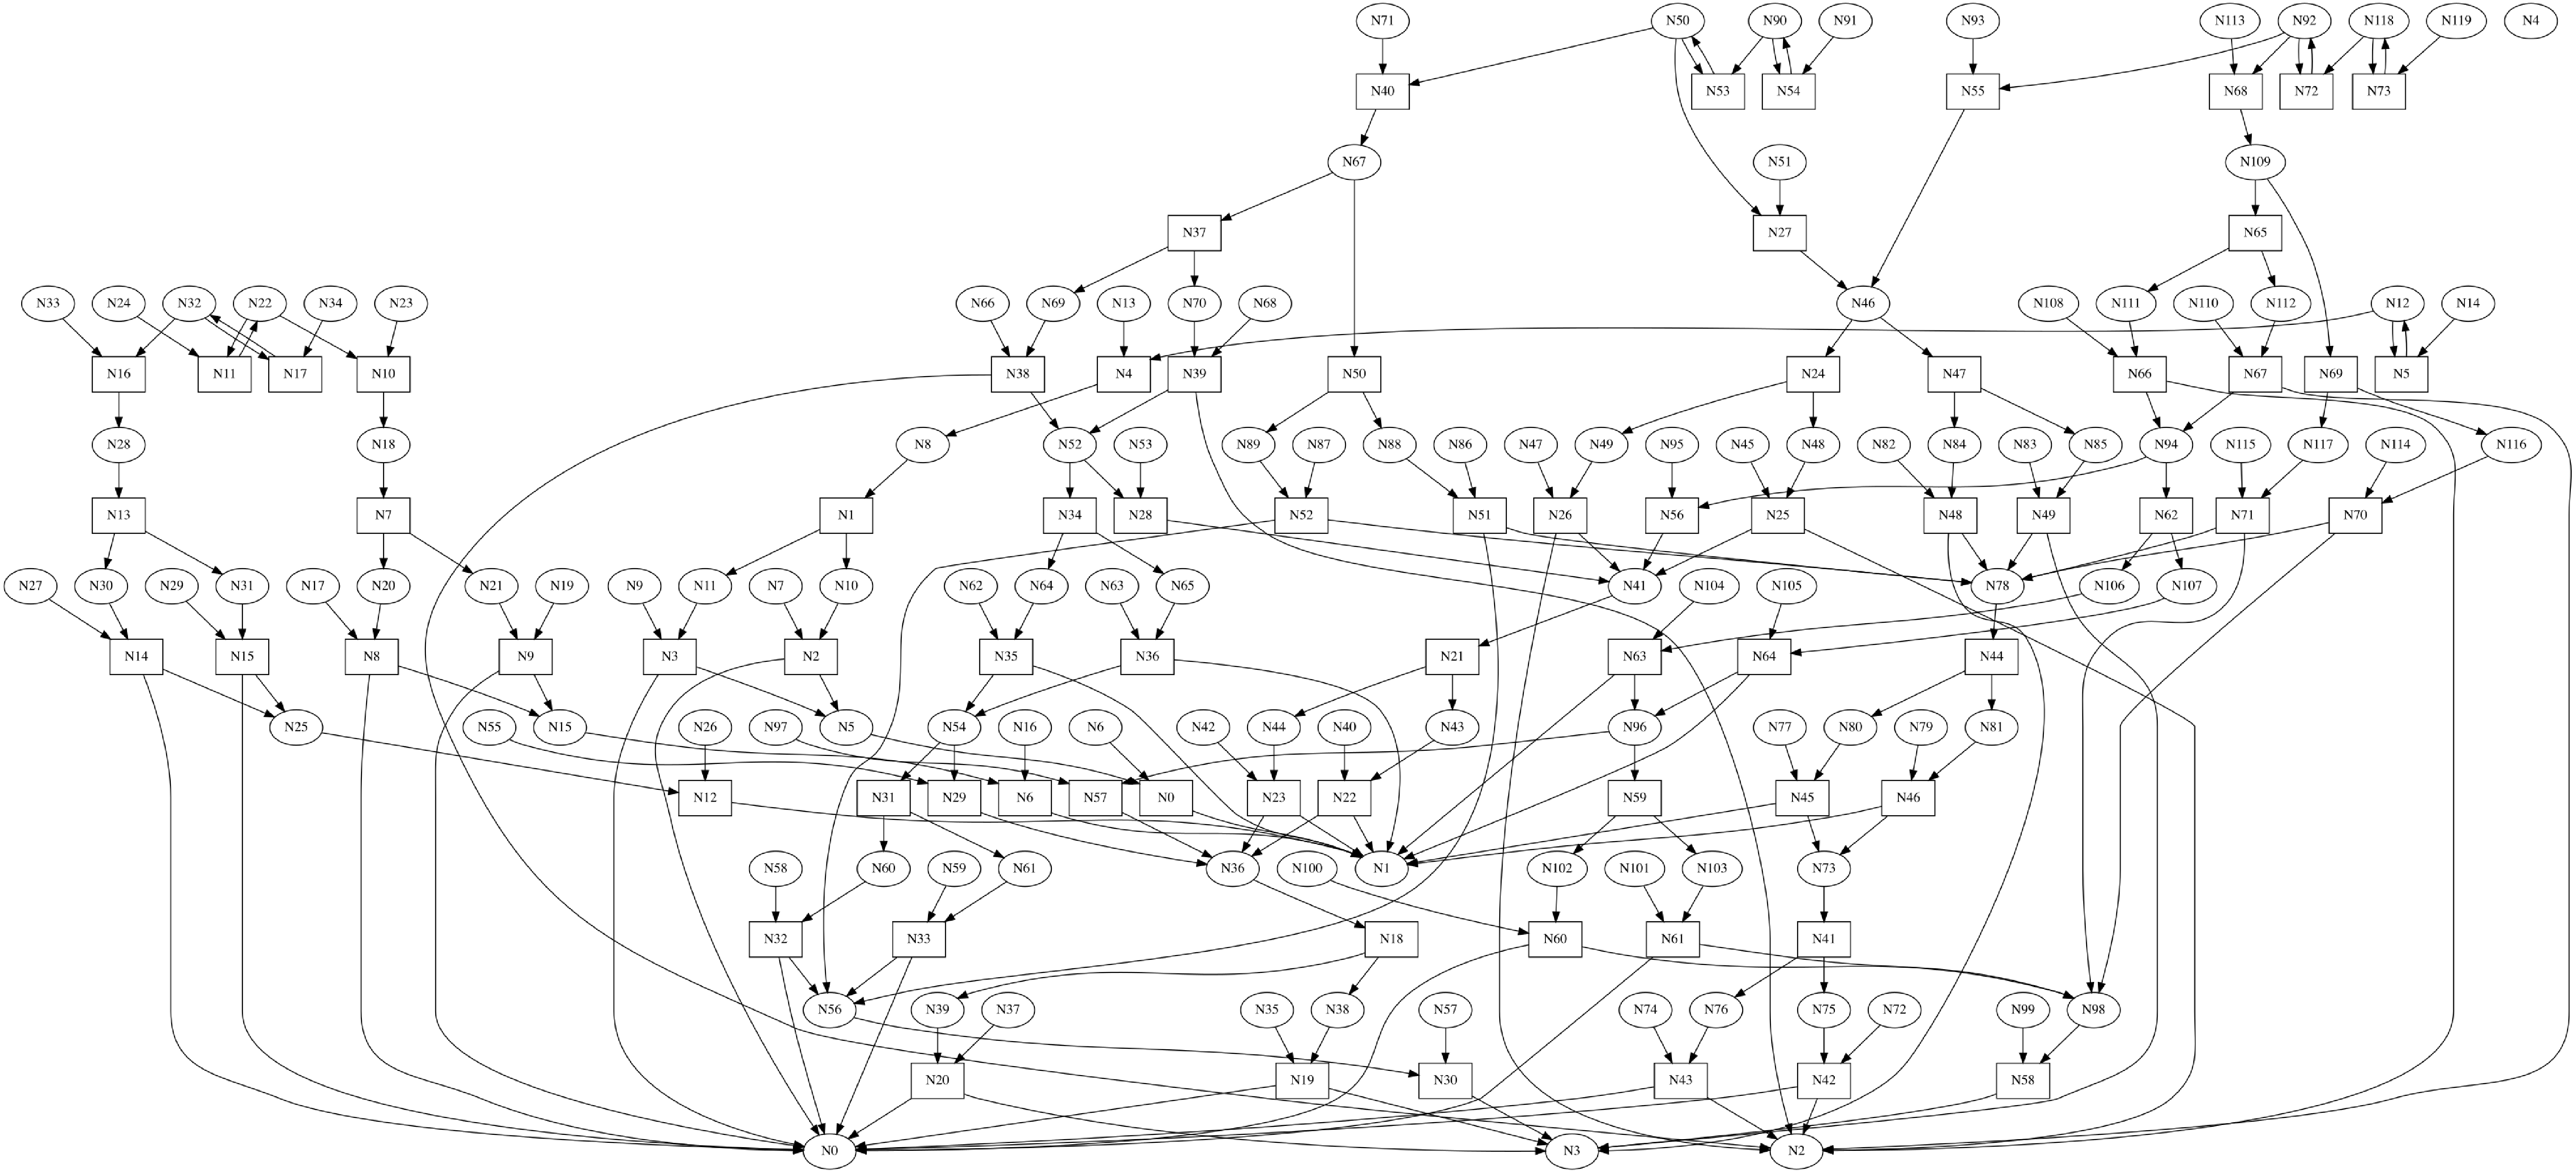
\includegraphics[width=\textwidth]{./imgs/ssb_graph.pdf}
  \caption{\label{fig:ssb_graph}A QDAG accumulated out of every node
    in the SSB TPC-H.}
\end{figure}

\section{Relation shapes}
\label{sec:relation_shapes}

In section \ref{sec:qnf} on QNFs we discussed the need to abstract away
information that pertains to the particular structure of a relation in
favor of semantic information that is rewrite and data
independent. Relation shapes cover the opposite need: they encode the
particular cardinality and shape of a relation at a specific point in
time.

A relation shape is a data structure that contains information about
the shape of the result of a query.

\begin{haskellcode}
  data RelationShape' e' =
    RelationShape
    { rsSchema :: [(e',ColumnProps)]
      ,rsUnique :: NEL.NonEmpty (NEL.NonEmpty e')
      ,rsSize :: RelationSize
    }

  type RelationShape e s = RelationShape' (ShapeSym e s)

  data ShapeSym e s =
    ShapeSym { planSymQnfName :: QNFName e s
      ,planSymQnfOriginal :: e
    }
    deriving (Show,Generic)
\end{haskellcode}

Focusing on the field \hask{rsUnique}, a shape contains 
all combinations of columns that comprise a unique
subtuple.  This is useful primarily to determine foreign key
joins. The expression

\[Q_1 := A \Join_{bId_A = id_B \land cId_A = id_C} (B \times C)\]

behaves like a foreign key join while the join when \(id_B\) is the
only element of the unique subtuple of \(B\) and \(id_C\) is the only
element of the unique subtuple of \(C\).

\[Q_2 := A \Join_{bId_A = id_B} (B \times C)\]

does not because for the expression\(B \times C\) neither \(id_B\) nor
\(id_C\) are unique on their own.  Only their combination
is. Therefore, the cardinality \(|Q_1|\) is at most the size of \(A\)
because each row of \(A\) matches at most one row of \(B \times C\).

So the unique subtuples are computed using the following rules:

\begin{itemize}
\item The set of unique subtuples of \(A \Join B\) is
  computed by concatenating all combinations of the unique subtuples
  of \(A\) and \(B\).
\item The unique subtuples of a selection, semijoin, antijoin, and limit are the same as the unique
  subtuples of the underlying relation.
\item The unique subtuples of a projection are the unique subtuples of
  the input that are entirely exposed.  The reader is reminded that
  FluiDB's notion of RA requires that there is at least one such
  unique subtuple, and that this requirement is facilitated by the
  query pre-processor.
\end{itemize}

The rest of the fields are maintained by \emph{shape propagators}.

\subsection{Shape propagators}
\label{sec:shape_propagators}

Shape propagators are based on the the idea of the propagator as first
introduced in \cite{sussmanArtPropagator2009} and analyzed more in
depth in \cite{hansonSoftwareDesignFlexibility2021a} and mentioned in
section \ref{sec:qdag}. Very briefly, a propagator network is a
hypergraph of cells containing mutable state and hyperedges as
multi-directional functions that, when triggered, update the state of
the connected cells so they are consistent with each other. The state
of each cell represents some information about a value (like a bound
or a probability distribution), and the propagator takes into account
the state of each cell and propagates that information to the other
cells (for example tightening their bound or finding a linear
combination of alternative values based on the certainty of
each). Kmett \cite{kmettPropagators2021} formalized the notion of
"information about a value" drawing from
\cite{kuperLVarsLatticebasedData2013} encoding it as a lattice with
\(\top\) meaning contradiction, and \(\bot\) meaning that there is no
information about the value. Then the new values of cells are being
joined ( \(\lor\) ) with the old ones and the value is updated to
reflect the combination of information. The example provided by Kmett
is each cell value being embedded in a 3 level lattice where the
bottom level is \hask{Nothing}, the middle level is \hask{Just x} and
the top level being a Haskell error (ironically denoted as \(\bot\) in
literature unrelated to propagators).

As the name of our propagator implementation suggests, our idea is to
correspond each cluster to a propagator to form a propagator network
that computes the shapes of the relations corresponding to n-nodes.

We model a propagator as a partial function that changes
the values at the edges of a cluster. Each cluster is equipped with a
propagator which, when triggered synchronizes the values at the edges
of the cluster. The partiality of the function stems from the fact
that it might detect irreconcilable inconsistencies between the cells
(see listing \ref{lst:acpropagator}). This conception of the
propagator departs slightly form the conception described in the paper
in that it clearly separates the \emph{cluster} as a data structure
that holds a fixed number of interdependent values, and the function
that updates the values in that cluster.

\begin{code}
  \begin{haskellcode}
    type ACPropagator a e s t n =
      EndoE e s (PropCluster a NodeRef e s t n)
    type EndoE e s x = x -> Either (AShowStr e s) x
    type ShapeCluster f e s t n =
      PropCluster (RelationShape e s) f e s t n
    type PropCluster a f e s t n =
      AnyCluster' (ShapeSym e s) (WMetaD (Defaulting a) f) t n
    newtype WMetaD a f b = WMetaD { unMetaD :: (a,f b)}
  \end{haskellcode}
  \caption{\label{lst:acpropagator}A propagator matches a cluster with
    shapes at the edges to the same kind of cluster with the shapes
    synchronized.}
\end{code}

Given a cluster with n-nodes at the edges, we look up the shape of each
node and add that to the cluster edge.  Once a cluster is triggered
and the values synchronized, those values are checked against the old
ones and for the ones that were updated we find the clusters in which
they participate and run the same process. The convergence of this
process is justified in \cite{kuperLVarsLatticebasedData2013}.

\subsection{Defaulting functor}

As mentioned, the cells of a propagator involve more structure than
raw values. Indeed, FluiDB wraps these values in a functor that we dub
as \emph{defaulting functor (DF)} to reason about the consistency of
the relation shape. In particular, we require that the cell can handle
cases where

\begin{itemize}
\item The shape is not computed yet, i.e., there is no information
  about the value.
\item The shape is inferred via the propagator network and is
therefore subject to change and
\item The shape stored in the cell corresponds to a materialized node
and other parts of the FluiDB's internal state depend on it.
\end{itemize}

The latter case is salient. Different logical plans can lead to
different, yet semantically equivalent as per the FluiDB RA.

The DF may hold up to two values (see listing
\ref{lst:defaulting_functor}).

\begin{itemize}
\item An empty DF means we have no information about the value.
\item A single value (the "default" value) corresponds to a derived
  shape that was computed using the propagator network. The default
  value is updated when propagators are triggered.
\item A full value exists alongside a default value and is constant
  through its lifetime as it matches the value of some state that is
  external to the propagator network, in our particular application it
  represents the shape of a materialized relation. Until that relation
  is deleted, and the full propagator is demoted to a defaulting one,
  the registered shape is not allowed to change.
\end{itemize}

\begin{code}
  \begin{haskellcode}
    data Defaulting a =
      DefaultingEmpty
      | DefaultingDef a
      | DefaultingFull a a
  \end{haskellcode}

  \caption{\label{lst:defaulting_functor}The defaulting functor definition.}
\end{code}

Since instances of the DF are meant to accommodate propagator values,
adhering to Kmett's approach to cell value maintenance, we define a
semilattice over the DF and define it in terms of a monoid (listing
\ref{lst:defaulting_semigroup} ).

Semigroups are not commutative, so we give meaning to the order. The
left operand of the semigroup operator is the newer value and the
right one is the older value. Therefore, the DF does not require all
the properties of the semilattice which is required to commutative and
associative. In general, the semigroup implemented by the underlying
type of the DF is taken to mean
\(\mathit{better} \diamond \mathit{backup}\), i.e. keep as much of the
left operand as possible unless the right operand is found to be
"better", for some definition of better. For example, when calculating
the cardinality we include a value of certainty between
\(\left[0,1\right]\).  A more certain right-hand cardinality is
preferred over a less certain left-hand side.

Bringing our attention to the implementation of the \hask{Def <> Full}
combination in the semigroup definition \ref{lst:defaulting_semigroup}
it is worth noting that it inverts the order of the combination of the
default values. The reason we do this is to give priority the the full
valued (materialized) nodes when propagating to their immediate
neighbors. We need this when committing an operator to the code
generation.

\begin{code}
  \begin{haskellcode}
    instance Semigroup a => Semigroup (Defaulting a) where
      DefaultingEmpty <> a = a
        a <> DefaultingEmpty = a
      DefaultingDef a <> DefaultingDef a' = DefaultingDef $ a <> a'
      DefaultingDef a <> DefaultingFull a' b' =
        DefaultingFull (a <> a') b'
      DefaultingFull a b <> DefaultingDef a' =
        DefaultingFull (a <> a') b
      DefaultingFull a b <> DefaultingFull a' _ =
        DefaultingFull (a' <> a) b

    instance Semigroup a => Monoid (Defaulting a) where
      mempty = DefaultingEmpty
  \end{haskellcode}

  \caption{\label{lst:defaulting_semigroup}The monoid define over the DF 
  is the right semilattice. A DF contains up  two values, the "default" and the "full" value.
  The "full" value refers to some property external to the defaulting functor, namely a 
  materialized relation, and therefore is not subject to change. The "default" value
  is gradually refined through monoidal combination. Combination of DFs is associative but not
  commutative: the right operand is expected to be the more recent one. Therefore
  we keep the left hand side "full" if we are combining two of them.}
\end{code}

When committing to a query plan, we are also committing to full values
for the defaulting values in the propagator cells. Every operator of
the plan corresponds to a relation shape propagator. When committing
an operator to the plan by translating it into C++ code, we promote
all the defaulting values at the edges. It is clear that the generated
code expects a certain data layout and therefore the \emph{full parts
of the values must be structurally consistent with each other}.

As we went over in the previous sections, however, the default values
are consistent with other default values of the same cluster
w.r.t. the amount of information they hold, but not w.r.t. the order
of the columns in the relation shape. Therefore, before promoting the
default functors to full functors by duplicating the default value to
fill both fields of the \hask{DefaultingFull} constructor, we trigger
the propagator to enforce full consistency between the
\hask{DefaultingDef} values.

The full part and the default part of the the defaulting value are not
necessarily structurally synchronized. We \emph{internally
synchronise} a cell before triggering the propagator to make sure we
maintain the consistency of the newly promoted cells with the already
existing full cells. It is notable that there is no formal guarantee that the propagator
will be able to create structurally consistent cells. In that case the
propagator will fail. Handling of this failure gracefully is beyond
the current scope of this work.

When an n-node is to be materialized, the corresponding defaulting
functor containing the value is \emph{promoted}.  Promotion of
propagators is copying the default value of a non-full prpagator to
the full state (listing \ref{lst:promote_defaulting}).


\begin{code}
  \begin{haskellcode}
    promoteDefaulting :: Defaulting a -> Defaulting a
    promoteDefaulting = \case
      DefaultingEmpty        -> DefaultingEmpty
      DefaultingDef x        -> DefaultingFull x x
      d@(DefaultingFull _ _) -> d
  \end{haskellcode}

  \caption{\label{lst:promote_defaulting}Promoting of defaulting functor happens
    during code generation when an n-node is materialized.}
\end{code}

\section{Summary and conclusion}

In this chapter we detailed how FluiDB processes queries. From
parsing to generating a graph of queries (QDAG) and inferring the
shapes of the relations in that graph. We also discussed different
conceptions of relational algebra that are used in FluiDB (normal RA
and QNF) and reverse operations. This will serve as a solid  on
which we can build the query planner and on top of the code generator.

There are a few shortcomings to this model that we have not yet
addressed that we plan to implement in later incarnations of
FluiDB. The most important ones being:

\begin{itemize}
\item As things stand, the QDAG will keep growing infinitely as new
  queries arrive and there is no obvious way to prune it while
  guaranteeing the materializability of all n-nodes.
\item There is no obvious path to supporting updates in the primary
  tables. There has been a lot of work on materialized view
  maintenance but most of it assumes that the primary tables are
  already materialized.
\end{itemize}
